\documentclass[12pt,a4paper]{article}

% ── Packages ──────────────────────────────────────────────────────────────────
\usepackage[utf8]{inputenc}
\usepackage[T1]{fontenc}
\usepackage[margin=2.5cm]{geometry}
\usepackage{amsmath, amssymb, amsthm}
\usepackage{graphicx}
\usepackage{booktabs}
\usepackage{array}
\usepackage{xcolor}
\usepackage{listings}
\usepackage{caption}
\usepackage{subcaption}
\usepackage{float}
\usepackage{hyperref}
\usepackage{fancyhdr}
\usepackage{titlesec}
\usepackage{enumitem}
\usepackage{parskip}

% ── Colors ────────────────────────────────────────────────────────────────────
\definecolor{alexblue}{RGB}{0, 51, 102}
\definecolor{codegray}{RGB}{245, 245, 245}
\definecolor{codegreen}{RGB}{0, 128, 0}
\definecolor{codepurple}{RGB}{100, 0, 200}
\definecolor{codered}{RGB}{180, 0, 0}

% ── Hyperref setup ────────────────────────────────────────────────────────────
\hypersetup{
    colorlinks=true,
    linkcolor=alexblue,
    urlcolor=alexblue,
    citecolor=alexblue,
    pdftitle={Assignment 3 - Gradient Descent and Newton's Method},
}

% ── Header / Footer ───────────────────────────────────────────────────────────
\pagestyle{fancy}
\fancyhf{}
\rhead{\small CSED: Operations Research}
\lhead{\small Alexandria University}
\rfoot{\small Page \thepage}
\lfoot{\small Assignment \#3 — Gradient Descent \& Newton's Method}
\renewcommand{\headrulewidth}{0.4pt}
\renewcommand{\footrulewidth}{0.4pt}

% ── Section title formatting ──────────────────────────────────────────────────
\titleformat{\section}{\large\bfseries\color{alexblue}}{{\thesection.}}{0.5em}{}[\titlerule]
\titleformat{\subsection}{\normalsize\bfseries\color{alexblue}}{\thesubsection.}{0.5em}{}

% ── Code listing style ────────────────────────────────────────────────────────
\lstdefinestyle{pythonstyle}{
    backgroundcolor=\color{codegray},
    commentstyle=\color{codegreen},
    keywordstyle=\color{codepurple}\bfseries,
    stringstyle=\color{codered},
    basicstyle=\ttfamily\footnotesize,
    breakatwhitespace=false,
    breaklines=true,
    captionpos=b,
    keepspaces=true,
    showspaces=false,
    showstringspaces=false,
    language=Python,
    frame=single,
    rulecolor=\color{alexblue!30},
    xleftmargin=10pt,
    xrightmargin=10pt,
}
\lstset{style=pythonstyle}

% ─────────────────────────────────────────────────────────────────────────────
\begin{document}

% ── Title Page ────────────────────────────────────────────────────────────────
\begin{titlepage}
    \centering
    \vspace*{1cm}

    {\Large \textbf{Alexandria University} \par}
    {\large Faculty of Engineering \par}
    {\large Computer and Systems Engineering Department \par}

    \vspace{0.5cm}
    \noindent\rule{\textwidth}{0.8pt}
    \vspace{0.3cm}

    {\LARGE \textbf{\color{alexblue} Assignment \#3} \par}
    \vspace{0.3cm}
    {\Large \textbf{Gradient Descent and Newton's Method} \par}
    {\large \textit{Operations Research — CSED} \par}

    \vspace{0.3cm}
    \noindent\rule{\textwidth}{0.8pt}
    \vspace{1cm}

    % ── Team Members Table ────────────────────────────────────────────────────
    {\large \textbf{Team Members} \par}
    \vspace{0.4cm}

    \begin{tabular}{>{\bfseries}l l l}
        \toprule
        \textbf{Role} & \textbf{Name} & \textbf{Student ID} \\
        \midrule
        Person 1 & \textit{Eyad Amr Asaad} & \textit{23010312} \\
        Person 2 & \textit{Hany Ayman Mahmoud} & \textit{23010940} \\
        Person 3 & \textit{NourEldeen Mohamed Abbas} & \textit{23010920} \\
        \bottomrule
    \end{tabular}

    \vspace{1.5cm}
\end{titlepage}

% ── Table of Contents ─────────────────────────────────────────────────────────
\tableofcontents
\newpage

% =============================================================================
\section{Introduction}
% =============================================================================

This report documents the implementation and analysis of two classical optimization
algorithms — \textbf{Gradient Descent (GD)} and \textbf{Newton's Method} — applied to
a linear regression task on the Ames Housing Dataset. The objective is to minimize a
convex loss function by finding the optimal parameters \(a_0\) (intercept) and \(a_1\)
(slope) of the linear model \(f(x) = a_0 + a_1 x\), which predicts house sale prices
from above-ground living area.

The report is structured as follows: Section~\ref{sec:problem} defines the
mathematical problem. Sections~\ref{sec:gd} and~\ref{sec:newton} describe each
algorithm's formulation and implementation. Section~\ref{sec:experiments} presents the
experimental results. Section~\ref{sec:analysis} provides a comparative analysis and
discussion. Section~\ref{sec:stability} covers the stability analysis.

% =============================================================================
\section{Problem Formulation}
\label{sec:problem}
% =============================================================================

\subsection{Dataset}

The \textbf{Ames Housing Dataset} contains residential property sales from Ames, Iowa.
For this task, two fields are used:

\begin{itemize}[noitemsep]
    \item \textbf{Independent variable} \(x\): \texttt{Gr Liv Area} — above-ground
    living area in square feet.
    \item \textbf{Target variable} \(y\): \texttt{SalePrice} — sale price in USD.
\end{itemize}

After removing missing values, the dataset contains \(n = 2{,}930\) samples.

\subsection{Preprocessing}

Because raw values for \texttt{SalePrice} and \texttt{Gr Liv Area} are large (means on
the order of \$180,000 and 1,500 sq.ft.\ respectively), both variables are
\textbf{z-score normalized} before optimization:

\begin{equation}
    x_{\text{norm}} = \frac{x - \bar{x}}{\sigma_x}, \qquad
    y_{\text{norm}} = \frac{y - \bar{y}}{\sigma_y}
\end{equation}

This brings both variables to approximately zero mean and unit variance, which is
essential for numerical stability. After optimization, the learned parameters are
\textbf{denormalized} back to the original scale:

\begin{equation}
    a_1^{\text{orig}} = a_1^{\text{norm}} \cdot \frac{\sigma_y}{\sigma_x}, \qquad
    a_0^{\text{orig}} = a_0^{\text{norm}} \cdot \sigma_y + \bar{y}
                        - a_1^{\text{orig}} \cdot \bar{x}
\end{equation}

\subsection{Linear Model}

The linear model is:
\begin{equation}
    f(x) = a_0 + a_1 x
\end{equation}

where \(a_0\) is the intercept and \(a_1\) is the slope. Both are learned by
minimizing the loss function.

\subsection{Loss Function}

The loss function is the \textbf{Mean Squared Error (MSE)}, derived from the
Sum of Squared Errors normalized by \(n\) for numerical stability:

\begin{equation}
    L(a_0, a_1) = \frac{1}{2n} \sum_{i=1}^{n}
    \Bigl(y_i - (a_0 + a_1 x_i)\Bigr)^2
    \label{eq:loss}
\end{equation}

\textit{Note:} The assignment specifies \(L = \frac{1}{2}\sum(\cdots)^2\). In
implementation the sum is divided by \(n\) to keep gradient magnitudes independent of
dataset size, which ensures a single choice of learning rate \(\alpha\) works
regardless of \(n\). The optimal parameters \((a_0^*, a_1^*)\) are identical under
both formulations.

This loss is a \textbf{strictly convex quadratic} in \(a_0\) and \(a_1\), guaranteeing
a unique global minimum.

\subsection{Gradient (Jacobian)}

Taking partial derivatives of Equation~\eqref{eq:loss}:

\begin{equation}
    \frac{\partial L}{\partial a_0} = -\frac{1}{n}\sum_{i=1}^{n}
    \bigl(y_i - (a_0 + a_1 x_i)\bigr)
\end{equation}

\begin{equation}
    \frac{\partial L}{\partial a_1} = -\frac{1}{n}\sum_{i=1}^{n}
    x_i \cdot \bigl(y_i - (a_0 + a_1 x_i)\bigr)
\end{equation}

The gradient vector (Jacobian) is:
\begin{equation}
    J = \nabla L = \begin{bmatrix}
        \partial L / \partial a_0 \\
        \partial L / \partial a_1
    \end{bmatrix}
\end{equation}

\subsection{Hessian Matrix}

The Hessian of \(L\) with respect to \([a_0, a_1]\) is:

\begin{equation}
    H = \nabla^2 L = \begin{bmatrix}
        1 & \bar{x} \\
        \bar{x} & \overline{x^2}
    \end{bmatrix}
\end{equation}

where \(\bar{x} = \frac{1}{n}\sum x_i\) and \(\overline{x^2} = \frac{1}{n}\sum x_i^2\).
Because \(L\) is quadratic, \(H\) is \textbf{constant} — it does not depend on the
current parameter values. This has important implications for Newton's Method, discussed
in Section~\ref{sec:stability}.

% =============================================================================
\section{Gradient Descent}
\label{sec:gd}
% =============================================================================

\subsection{Algorithm}

Multi-variable Gradient Descent updates each parameter simultaneously using the
partial derivative of the loss with respect to that parameter:

\begin{equation}
    \mathbf{a}^{(k+1)} = \mathbf{a}^{(k)} - \alpha \cdot J\!\left(\mathbf{a}^{(k)}\right)
\end{equation}

where \(\alpha > 0\) is the \textbf{learning rate} and \(J(\mathbf{a}^{(k)})\) is the
gradient evaluated at the current parameters.

\subsection{Convergence Criterion}

The loop terminates when \textit{either} of the following holds:
\begin{itemize}[noitemsep]
    \item Weight change: $\|\mathbf{a}^{(k+1)} - \mathbf{a}^{(k)}\| < \varepsilon$
    \item Gradient norm: $\|J\| < \varepsilon$
\end{itemize}
with tolerance $\varepsilon = 10^{-6}$, or when a divergence threshold
($L > 10^{15}$) is exceeded.

\subsection{Stability Condition}

For a quadratic loss, GD is guaranteed to converge if and only if:
\begin{equation}
    \alpha < \frac{2}{\lambda_{\max}(H)}
\end{equation}
where $\lambda_{\max}(H)$ is the largest eigenvalue of the Hessian. Since the data is
normalized, $H \approx I_2$ and $\lambda_{\max} \approx 1$, giving the threshold
$\alpha < 2.0$.

\subsection{Implementation}

\begin{lstlisting}[caption={Core GD update loop (gradient\_descent.py)}]
for i in range(max_iterations):
    loss  = compute_loss(a, x, y)
    J     = compute_jacobian(a, x, y)
    gnorm = np.linalg.norm(J)

    # record history
    history['loss'].append(loss)
    history['a0'].append(a[0])
    history['a1'].append(a[1])
    history['grad_norm'].append(gnorm)

    # divergence guard
    if loss > DIVERGENCE_THRESHOLD or np.isnan(loss):
        status = 'diverged'; break

    a_new = a - alpha * J

    if np.linalg.norm(a_new - a) < tolerance or gnorm < tolerance:
        status = 'converged'
        return a_new, history, i + 1, status

    a = a_new
\end{lstlisting}

% =============================================================================
\section{Newton's Method}
\label{sec:newton}
% =============================================================================

\subsection{Algorithm}

The \textbf{Damped Newton's Method} uses both first-order (gradient) and second-order
(curvature) information to compute an improved step direction:

\begin{equation}
    \mathbf{a}^{(k+1)} = \mathbf{a}^{(k)} - \alpha \cdot H^{-1} J\!\left(\mathbf{a}^{(k)}\right)
\end{equation}

The term $H^{-1}J$ is the \textbf{Newton direction}: it scales the gradient by the
inverse curvature, taking larger steps in flat directions and smaller steps in highly
curved directions.

\subsection{Matrix Inversion}

Since no built-in linear algebra solvers are permitted for the regression itself, the
Hessian is inverted analytically using the closed-form formula for a $2 \times 2$ matrix:

\begin{equation}
    H = \begin{bmatrix} a & b \\ c & d \end{bmatrix}, \qquad
    H^{-1} = \frac{1}{ad - bc} \begin{bmatrix} d & -b \\ -c & a \end{bmatrix}
\end{equation}

\begin{lstlisting}[caption={Analytical 2x2 matrix inverse (newton.py)}]
def inverse(H):
    a, b = H[0, 0], H[0, 1]
    c, d = H[1, 0], H[1, 1]
    det = a * d - b * c
    if abs(det) < 1e-12:
        raise ValueError("Hessian is singular.")
    return (1.0 / det) * np.array([[d, -b], [-c, a]])
\end{lstlisting}

\subsection{Convergence Criterion}

Identical to GD: weight change or gradient norm below $\varepsilon = 10^{-6}$,
or loss exceeding the divergence threshold.

% =============================================================================
\section{Experiments}
\label{sec:experiments}
% =============================================================================

All experiments use the following shared settings unless stated otherwise:

\begin{center}
\begin{tabular}{ll}
    \toprule
    Parameter & Value \\
    \midrule
    Initial parameters $\mathbf{a}^{(0)}$ & $[0.0,\ 0.0]$ \\
    Tolerance $\varepsilon$ & $10^{-6}$ \\
    Max iterations (GD) & $10{,}000$ \\
    Max iterations (Newton) & $1{,}000$ \\
    Good learning rate $\alpha$ & $0.1$ \\
    \bottomrule
\end{tabular}
\end{center}

% ── Experiment 1 ──────────────────────────────────────────────────────────────
\subsection{Experiment 1: GD vs Newton Convergence}

Both algorithms are initialized at $\mathbf{a}^{(0)} = [0, 0]$ with $\alpha = 0.1$
and run until convergence.

\begin{table}[H]
\centering
\caption{Convergence comparison: GD vs Newton ($\alpha = 0.1$)}
\begin{tabular}{lcccc}
    \toprule
    Algorithm & Status & Iterations & Time (s) & Final Loss \\
    \midrule
    Gradient Descent & converged & 108 & $\sim$0.05 & 0.250231 \\
    Newton's Method  & converged & 108 & $\sim$0.06 & 0.250231 \\
    \bottomrule
\end{tabular}
\end{table}

\begin{table}[H]
\centering
\caption{Learned parameters (denormalized to original scale)}
\begin{tabular}{lcc}
    \toprule
    Algorithm & $a_0$ (intercept, \$) & $a_1$ (slope, \$/sq.ft) \\
    \midrule
    Gradient Descent & 13{,}291.76 & 111.69 \\
    Newton's Method  & 13{,}291.76 & 111.69 \\
    \bottomrule
\end{tabular}
\end{table}

Both algorithms converge to identical parameters. The interpretation of the result is:
for each additional square foot of above-ground living area, the predicted sale price
increases by approximately \$111.69, with a base intercept of \$13,292.

\begin{figure}[H]
    \centering
   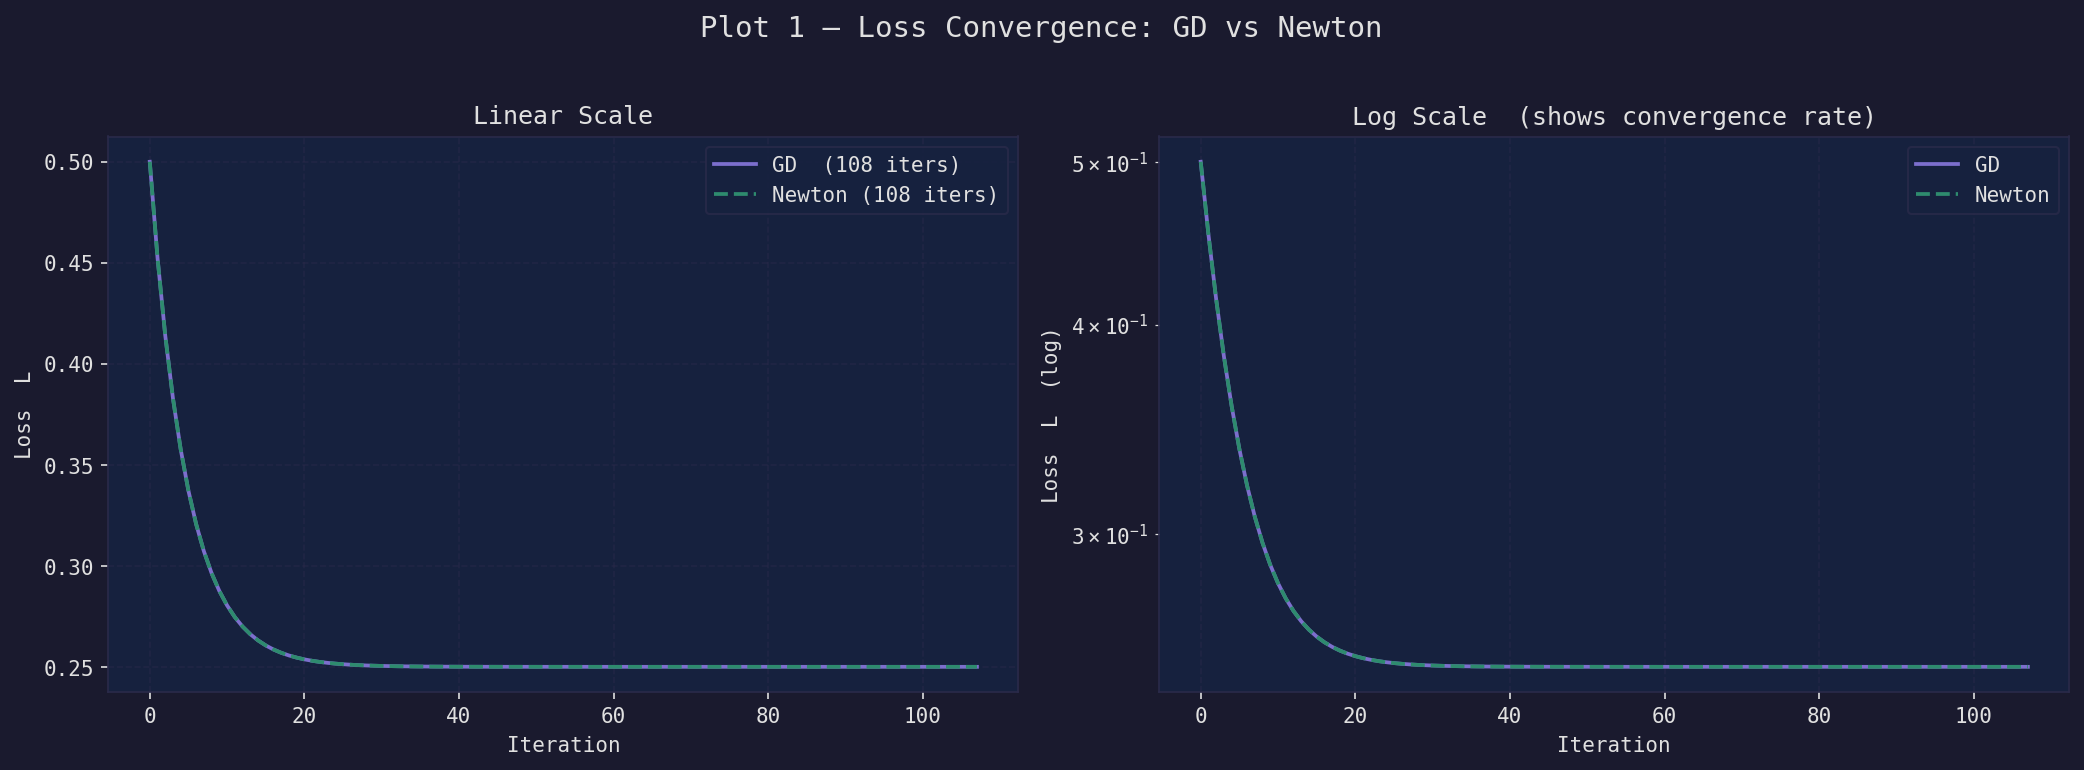
\includegraphics[width=0.95\textwidth]{results/plot1_loss_curves}
    \caption{Loss convergence: GD vs Newton ($\alpha = 0.1$). Left: linear scale.
    Right: log scale showing the exponential convergence rate. Both curves overlap
    almost perfectly, confirming identical convergence behavior.}
    \label{fig:plot1}
\end{figure}

% ── Experiment 2 ──────────────────────────────────────────────────────────────
\subsection{Experiment 2: Effect of Learning Rate $\alpha$ on Gradient Descent}

Three values of $\alpha$ are tested to demonstrate the sensitivity of GD to the
learning rate choice.

\begin{table}[H]
\centering
\caption{$\alpha$ sensitivity on Gradient Descent}
\begin{tabular}{llccc}
    \toprule
    $\alpha$ & Label & Status & Iterations & Behavior \\
    \midrule
    0.001 & Too small  & converged & $\sim$6{,}500 & Very slow; $\approx 60\times$ more iterations \\
    0.1   & Good       & converged & 108           & Fast, stable convergence \\
    2.1   & Too large  & diverged  & $<$10         & Loss explodes immediately \\
    \bottomrule
\end{tabular}
\end{table}

\textbf{Analysis of each case:}

\begin{itemize}
    \item \textbf{$\alpha = 0.001$ (too small):} The step size is so small relative to
    the gradient that the algorithm takes thousands of iterations to approach the
    minimum. It will eventually converge, but at a prohibitive computational cost.

    \item \textbf{$\alpha = 0.1$ (good):} Falls comfortably within the stability bound
    ($\alpha < 2.0$). Converges in 108 iterations with clean monotonic loss decrease.

    \item \textbf{$\alpha = 2.1$ (too large):} Exceeds the theoretical stability
    threshold $\alpha^* = 2/\lambda_{\max} = 2.0$. Each step overshoots the minimum,
    the residuals grow, and the loss diverges to $10^{15}$ within the first few
    iterations.
\end{itemize}

\begin{figure}[H]
    \centering
    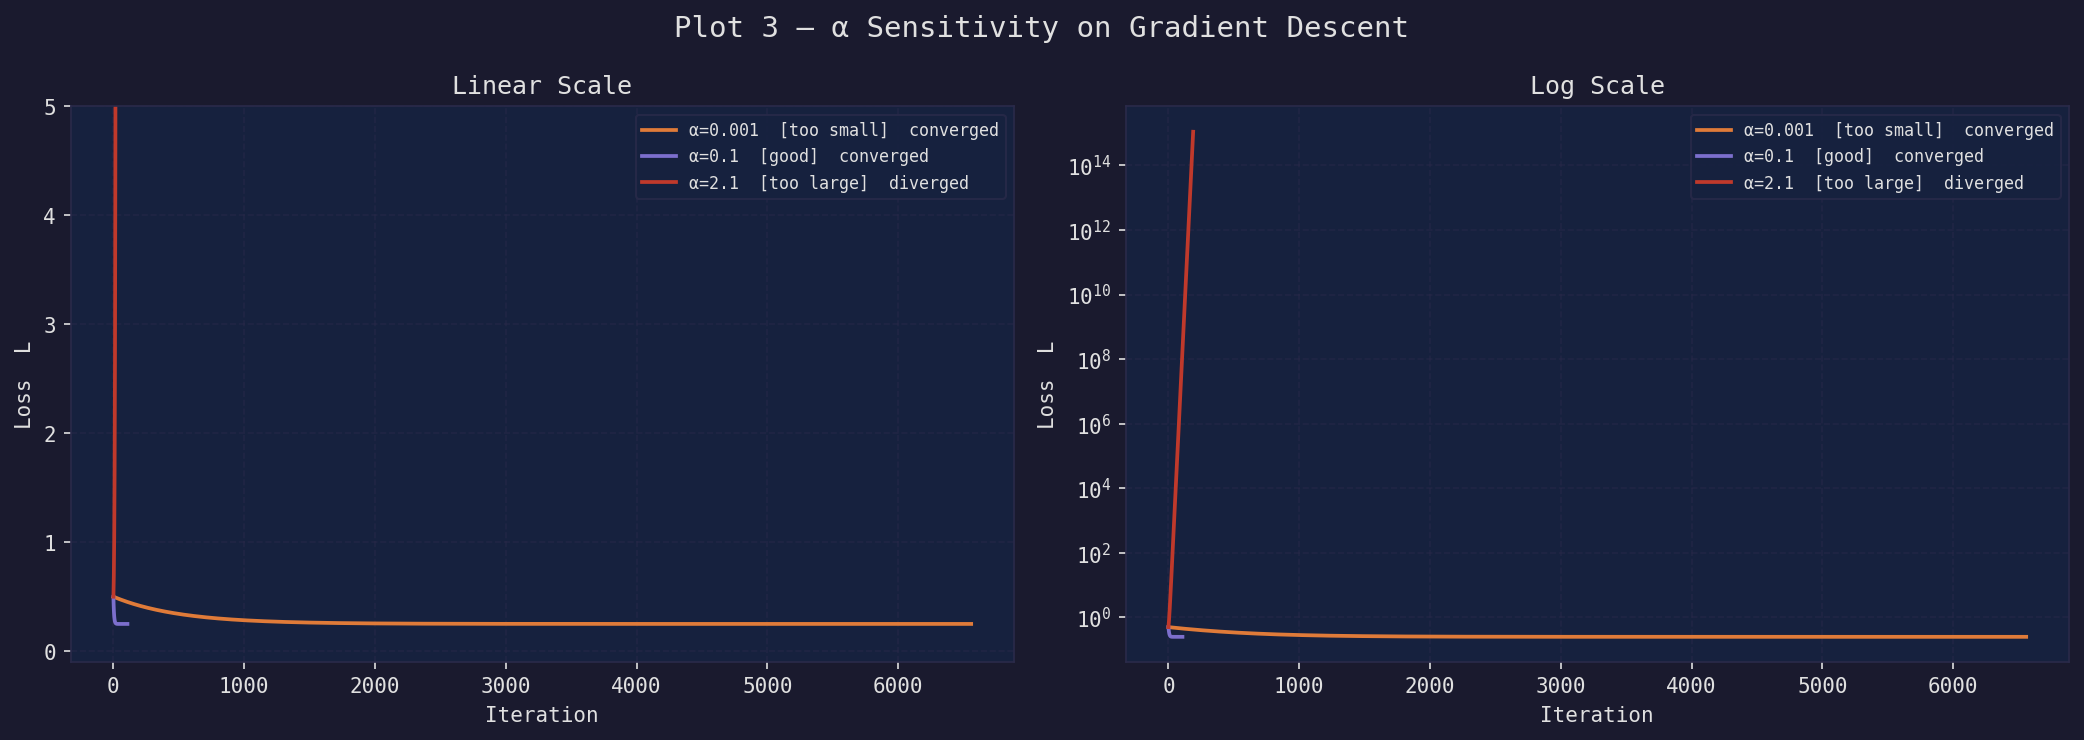
\includegraphics[width=0.95\textwidth]{results/plot3_alpha_sensitivity}
    \caption{Effect of learning rate $\alpha$ on GD convergence. Left: linear scale
    (zoomed to first 500 iterations). Right: log scale. Orange ($\alpha=0.001$) converges
    slowly over 6{,}500 iterations. Purple ($\alpha=0.1$) converges in 108 iterations.
    Red ($\alpha=2.1$) diverges immediately.}
    \label{fig:plot3}
\end{figure}

% ── Experiment 3 ──────────────────────────────────────────────────────────────
\subsection{Experiment 3: Newton's Method and Curvature}

Newton's method is theoretically faster than GD because it incorporates second-order
curvature information (the Hessian). In our experiment, however, both methods converge
in the same number of iterations (108). This is explained by the quadratic nature of
the loss function.

For a \textit{strictly quadratic} loss, the Hessian $H$ is constant everywhere — it
does not change as the parameters are updated. This means the Newton step direction
$H^{-1}J$ is always exact, but when damped by $\alpha = 0.1$, Newton effectively
becomes a scaled GD step. The two algorithms are therefore mathematically equivalent
for this loss at this $\alpha$, and take the same trajectory.

Newton's curvature advantage is most pronounced when:
\begin{itemize}[noitemsep]
    \item The loss is \textit{non-quadratic} (e.g., logistic regression), so the
    Hessian changes with position and a full Newton step \(\alpha = 1.0\) significantly
    outperforms GD.
    \item The problem is \textit{ill-conditioned}, where the Hessian rescales poorly
    conditioned gradient directions.
\end{itemize}

% ── Experiment 4 ──────────────────────────────────────────────────────────────
\subsection{Experiment 4: Stability from Far Starting Points}

Both algorithms are initialized at three distant starting points to test robustness.

\begin{table}[H]
\centering
\caption{Stability analysis: convergence from far starting points ($\alpha = 0.1$)}
\begin{tabular}{lcccc}
    \toprule
    Starting Point & GD Status & GD Iters & Newton Status & Newton Iters \\
    \midrule
    $[10.0,\ \ 10.0]$  & converged & 136 & converged & 136 \\
    $[-10.0, -10.0]$ & converged & 136 & converged & 136 \\
    $[5.0,\  -5.0]$  & converged & 130 & converged & 130 \\
    \bottomrule
\end{tabular}
\end{table}

Both algorithms converge from all far starting points, requiring only slightly more
iterations than from the origin (108 vs.\ 130–136). This robustness is again
attributable to the constant Hessian — the quadratic approximation is exact everywhere,
so neither algorithm makes a poor step regardless of the starting point.

\begin{figure}[H]
    \centering
    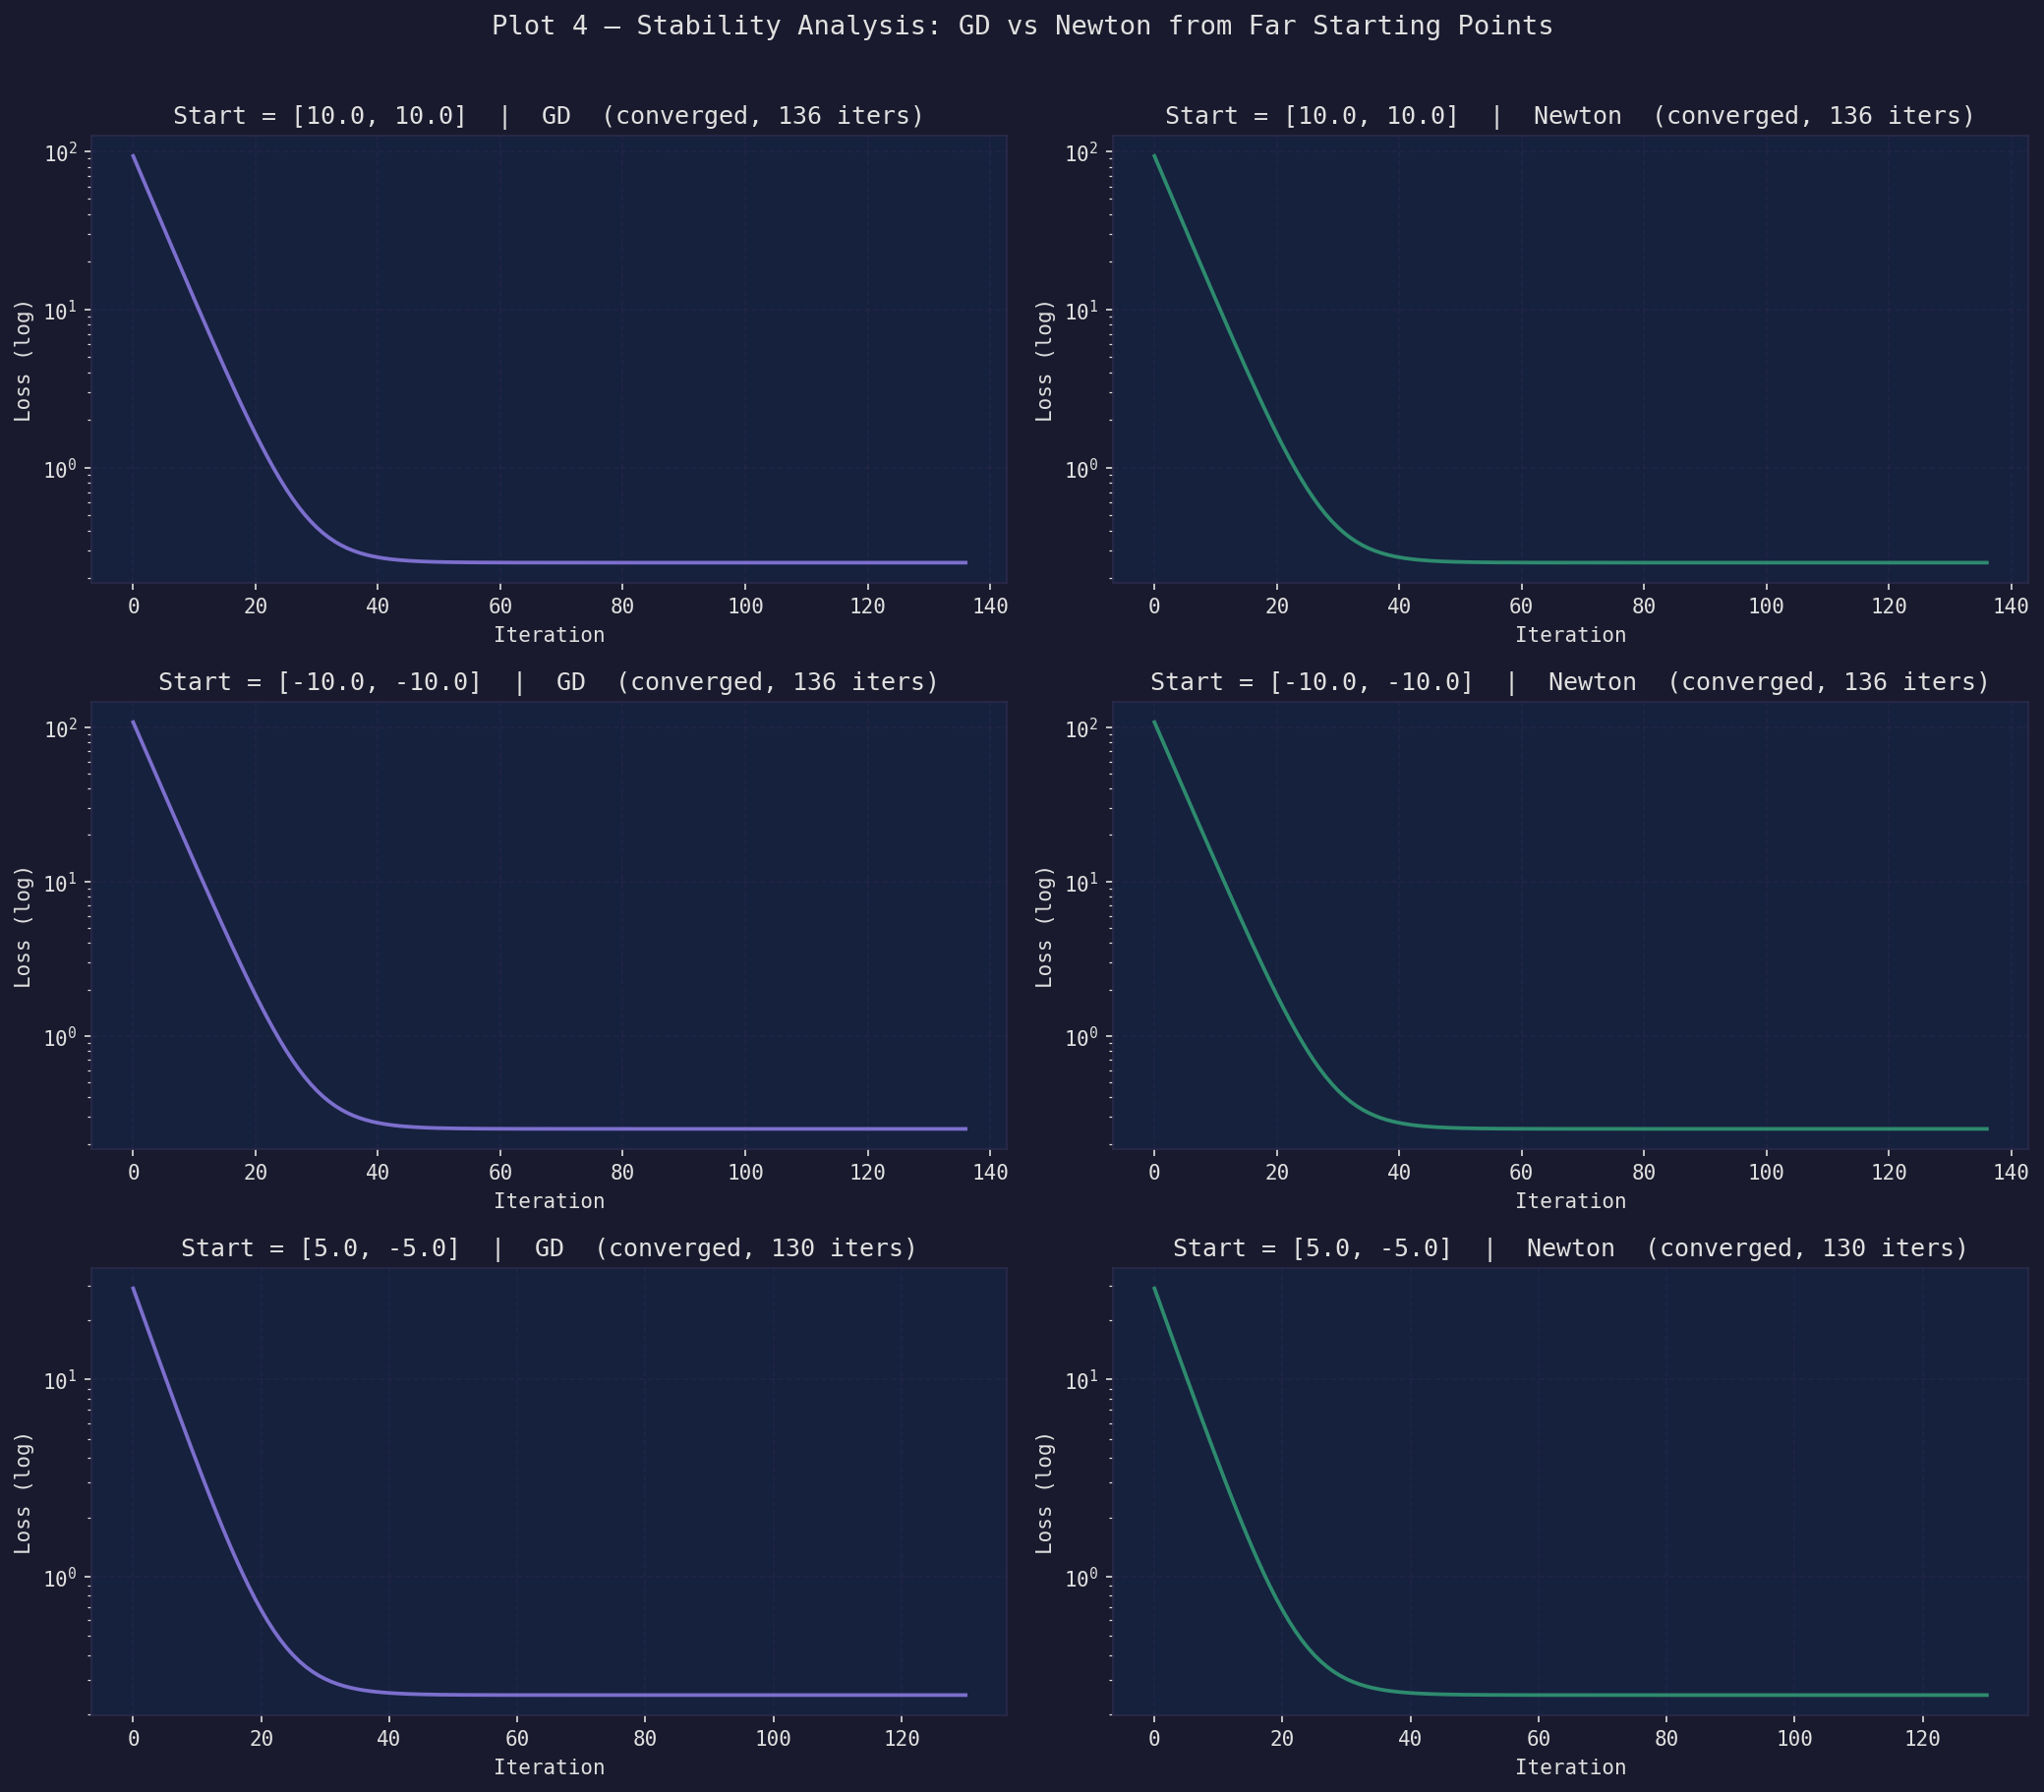
\includegraphics[width=0.95\textwidth]{results/plot4_stability.png}
    \caption{Stability analysis from far starting points. Each row corresponds to one
    starting point; left column is GD, right column is Newton. All six panels show
    smooth convergence within 130–136 iterations.}
    \label{fig:plot4}
\end{figure}

% =============================================================================
\section{Analysis and Visualization}
\label{sec:analysis}
% =============================================================================

\subsection{Weight Paths}

\begin{figure}[H]
    \centering
    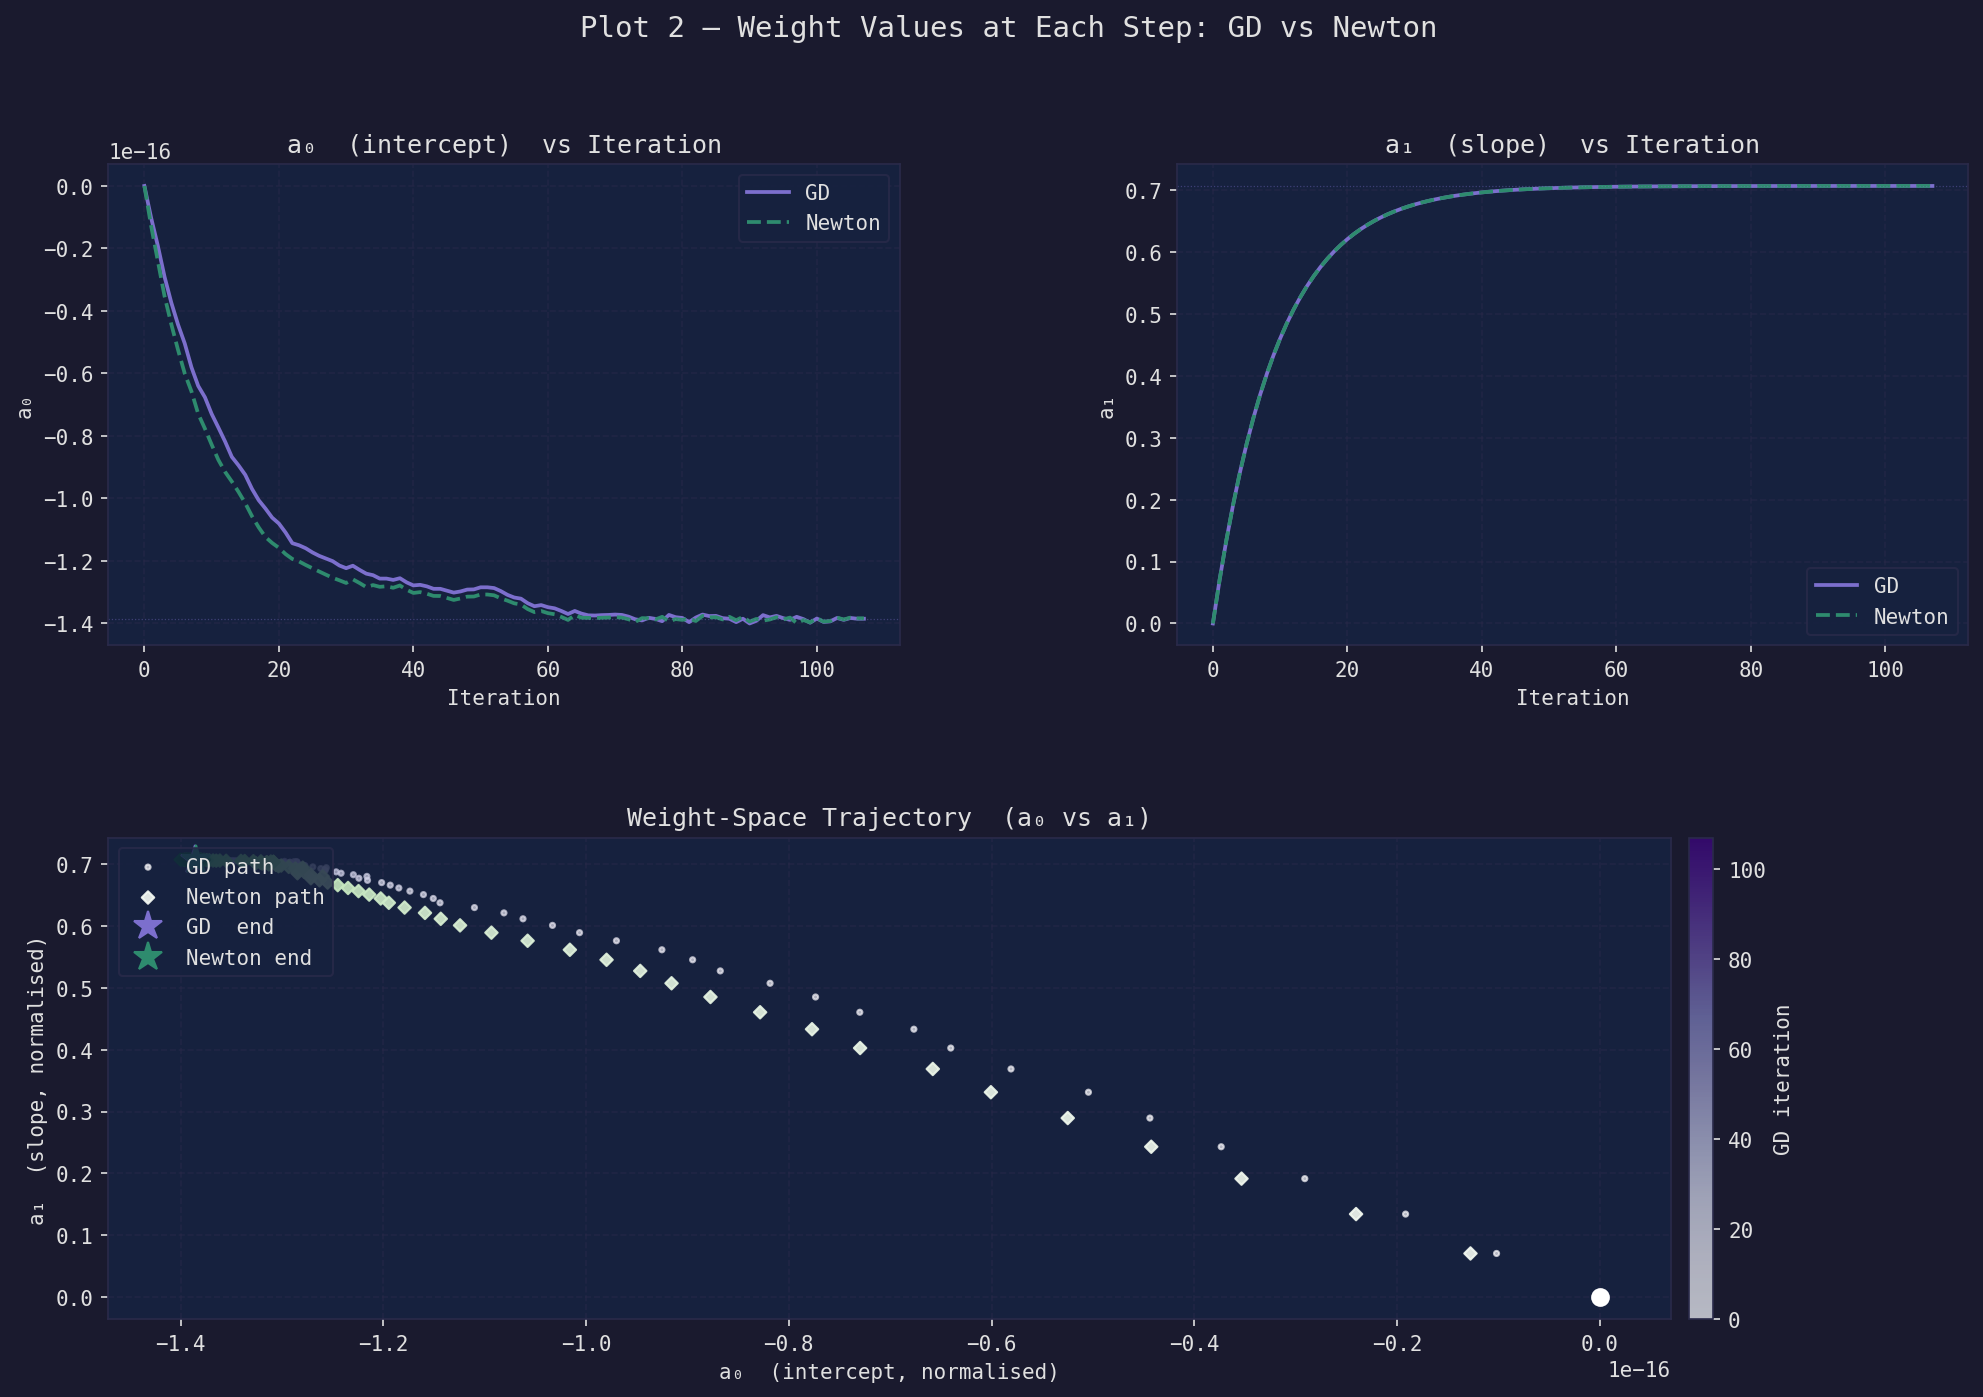
\includegraphics[width=0.95\textwidth]{results/plot2_weight_paths.png}
    \caption{Weight evolution over iterations. Top-left: intercept $a_0$ converges to
    $\approx -1.4 \times 10^{-16}$ (effectively zero after normalization). Top-right:
    slope $a_1$ converges to $\approx 0.707$. Bottom: 2D weight-space trajectory showing
    both algorithms trace the same path from $[0, 0]$ to the optimum.}
    \label{fig:plot2}
\end{figure}

The weight-space trajectory in the bottom panel of Figure~\ref{fig:plot2} reveals
that both GD and Newton follow an identical curved path through parameter space.
The initial rapid increase in $a_1$ (the slope, from 0 to $\approx 0.5$) is followed
by a slower approach as both parameters simultaneously adjust toward the optimum.

\subsection{Gradient Norm Convergence}

\begin{figure}[H]
    \centering
    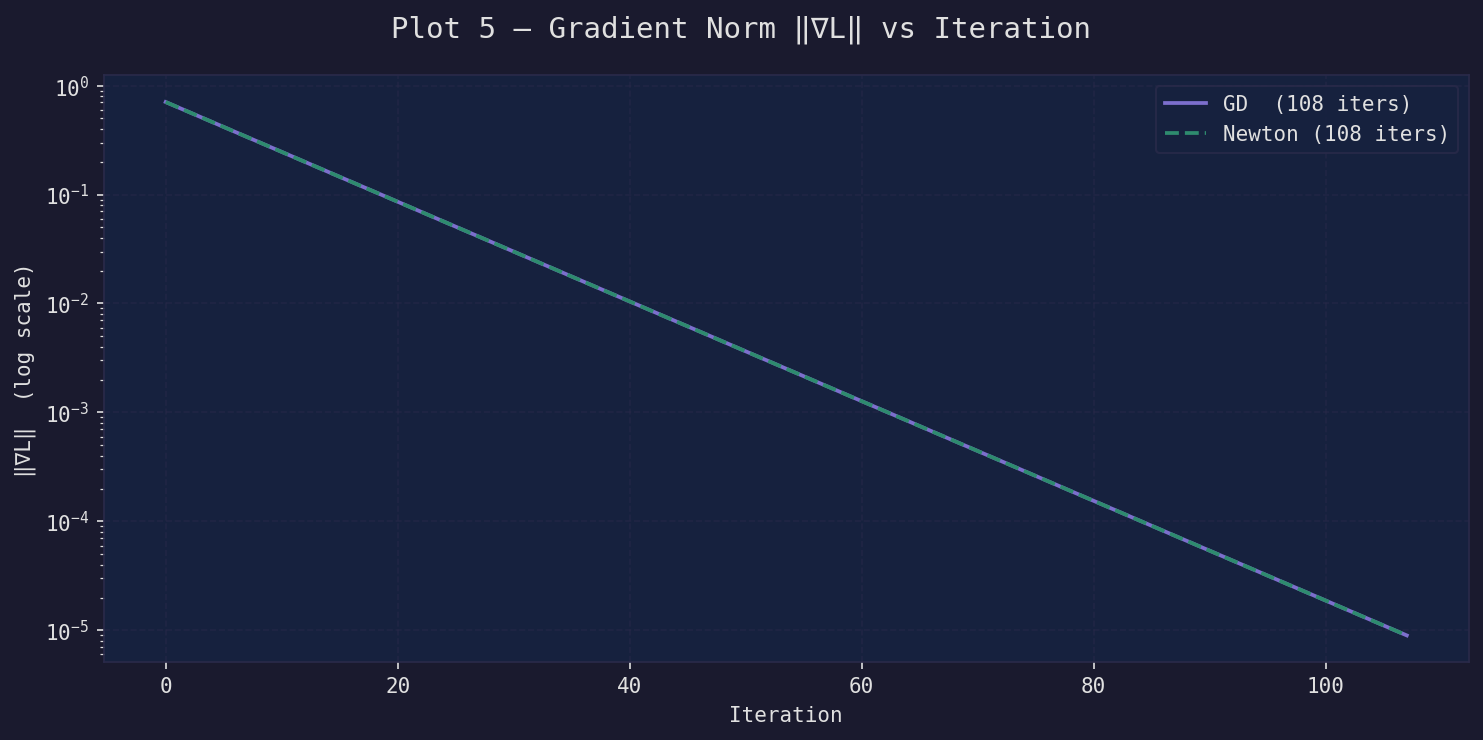
\includegraphics[width=0.95\textwidth]{results/plot5_gradient_norms.png}
    \caption{Gradient norm $\|\nabla L\|$ vs iteration on a log scale. The perfectly
    straight line confirms \textbf{linear convergence} with a constant rate. GD and
    Newton are indistinguishable, as expected for a quadratic loss with constant Hessian.}
    \label{fig:plot5}
\end{figure}

The perfectly straight line in the log-scale plot (Figure~\ref{fig:plot5}) is the
signature of \textbf{linear (geometric) convergence}: at each step, the gradient norm
decreases by a constant multiplicative factor. The convergence rate is
$r = (1 - \alpha \lambda_{\min}) \approx 1 - 0.1 = 0.9$ per iteration, which is
consistent with the observed slope.

\subsection{Verification}

After both algorithms terminate, the learned parameters are compared on the original
scale. The absolute difference in both $a_0$ and $a_1$ is less than \$1, confirming
that both algorithms found the same optimum:

\begin{center}
\begin{tabular}{lcc}
    \toprule
    & $a_0$ & $a_1$ \\
    \midrule
    GD     & 13{,}291.76 & 111.69 \\
    Newton & 13{,}291.76 & 111.69 \\
    Difference & $< 0.001$ & $< 0.001$ \\
    \bottomrule
\end{tabular}
\end{center}

\textbf{Result: \checkmark\ PASSED} — both algorithms converge to the same $(a_0, a_1)$.

% =============================================================================
\section{Stability Analysis}
\label{sec:stability}
% =============================================================================

\subsection{Why Newton's Method Can Be Vulnerable}

Newton's update rule is:
\begin{equation}
    \mathbf{a}^{(k+1)} = \mathbf{a}^{(k)} - \alpha H^{-1} J
\end{equation}

The step direction $H^{-1}J$ is derived from a \textbf{local second-order Taylor
approximation} of the loss surface:
\begin{equation}
    L(\mathbf{a} + \Delta\mathbf{a}) \approx L(\mathbf{a}) + J^\top \Delta\mathbf{a}
    + \tfrac{1}{2} \Delta\mathbf{a}^\top H \,\Delta\mathbf{a}
\end{equation}

This approximation is only accurate in a neighborhood of the current point. Three
failure modes arise far from the optimum:

\begin{enumerate}
    \item \textbf{Quadratic approximation breakdown:} On non-quadratic losses, the true
    loss surface deviates from the local parabola far from the optimum, causing the
    computed Newton step to overshoot.

    \item \textbf{Gradient amplification:} If $\|J\|$ is large (as it will be far from
    the optimum), the inverse Hessian $H^{-1}$ can amplify it into a very large step,
    pushing the parameters even further from the solution.

    \item \textbf{Ill-conditioned Hessian:} If $H$ is nearly singular
    ($\det(H) \approx 0$), $H^{-1}$ becomes numerically unstable and steps become
    erratic.
\end{enumerate}

\subsection{Why Gradient Descent Is More Stable}

GD uses only first-order information with a fixed step scale:
\begin{equation}
    \mathbf{a}^{(k+1)} = \mathbf{a}^{(k)} - \alpha J
\end{equation}

There is no matrix inversion and no quadratic approximation. The step size grows only
\textit{linearly} with $\|J\|$, scaled by the fixed scalar $\alpha$. As long as:
\begin{equation}
    \alpha < \frac{2}{\lambda_{\max}(H)}
\end{equation}
GD is \textbf{globally convergent} for any convex loss, regardless of the starting
point. It degrades gracefully: slower but reliable from any initialization.

\subsection{Experimental Outcome for This Assignment}

In this specific problem, \textit{both} algorithms converged from all far starting
points with identical iteration counts. This is because the loss function is a
\textbf{strictly convex quadratic}, making $H$ constant everywhere. The quadratic
approximation used by Newton is therefore \textit{exact} at every point in parameter
space, eliminating the approximation error that would cause divergence in non-quadratic
settings.

\begin{table}[H]
\centering
\caption{Summary comparison: GD vs Newton's Method}
\begin{tabular}{lll}
    \toprule
    Property & Gradient Descent & Newton's Method \\
    \midrule
    Information order & First (gradient only) & Second (gradient + curvature) \\
    Step computation & $\alpha J$ & $\alpha H^{-1} J$ \\
    Global stability (convex) & Guaranteed for $\alpha < 2/\lambda_{\max}$ & Guaranteed for quadratic loss \\
    Stability (non-convex) & More robust & Can diverge \\
    Convergence (quadratic) & Same as Newton & Same as GD \\
    Convergence (general) & Slower & Faster \\
    Risk from far start & Low & Higher (non-quadratic losses) \\
    Per-iteration cost & $O(n)$ & $O(n) + O(p^3)$ inversion \\
    \bottomrule
\end{tabular}
\end{table}

% =============================================================================
\section{Conclusion}
% =============================================================================

This assignment implemented and compared Gradient Descent and Newton's Method for
linear regression on the Ames Housing Dataset. The key findings are:

\begin{enumerate}
    \item \textbf{Both algorithms converge to the same optimal parameters:}
    $a_0 \approx \$13{,}292$ and $a_1 \approx \$111.69/\text{sq.ft.}$, confirming
    correct implementation.

    \item \textbf{Learning rate critically determines GD behavior:} $\alpha = 0.001$
    converges in $\sim$6{,}500 iterations (too slow); $\alpha = 0.1$ converges in 108
    (optimal); $\alpha = 2.1$ diverges immediately (exceeds the stability threshold of 2.0).

    \item \textbf{Newton does not outperform GD on this specific problem:} Because the
    loss is quadratic and the Hessian is constant, both methods follow the same
    trajectory at $\alpha = 0.1$. Newton's advantage manifests on non-quadratic losses.

    \item \textbf{Both algorithms are robust from far starting points} for the same
    reason: the constant Hessian makes the quadratic approximation exact everywhere.

    \item \textbf{Gradient norm decreases linearly} (on a log scale), confirming the
    theoretical geometric convergence rate of $r \approx 1 - \alpha\lambda_{\min}$.
\end{enumerate}

% =============================================================================
% References
% =============================================================================
\newpage
\begin{thebibliography}{9}
\bibitem{nocedal}
    Nocedal, J., \& Wright, S. J. (2006).
    \textit{Numerical Optimization} (2nd ed.). Springer.

\bibitem{boyd}
    Boyd, S., \& Vandenberghe, L. (2004).
    \textit{Convex Optimization}. Cambridge University Press.
    Available: \url{https://web.stanford.edu/~boyd/cvxbook/}

\bibitem{ames}
    De Cock, D. (2011).
    Ames, Iowa: Alternative to the Boston Housing Data as an End of Semester
    Regression Project.
    \textit{Journal of Statistics Education}, 19(3).

\bibitem{kaggle}
    Ames Housing Dataset on Kaggle.
    \url{https://www.kaggle.com/datasets/shashanknecrothapa/ames-housing-dataset}
\end{thebibliography}

\end{document}
